\documentclass[parskip=full]{scrartcl}

\usepackage[utf8]{inputenc}			% Umlaute, Sonderzeichen
\usepackage[ngerman]{babel}			% deutsche Sprache
\usepackage{enumitem}				% Listen
\usepackage{graphicx}				% Grafiken
\usepackage{hyperref}				% Hyperlinks
\usepackage[nonumberlist]{glossaries}		% Glossar
\usepackage{amsmath}
\usepackage{pdfpages}				% PDF einbinden


\makenoidxglossaries



\subject{Benutzerhandbuch}
\title{Handbuch zur Benutzung der Anwendung "FreeJDAQ"}
\subtitle{Version 1.0.0}
\author{David Gawron \and Stefan Geretschläger \and Leon Huck \and Jan Küblbeck \and Linus Ruhnke}
\date{\today}


\begin{document}

\maketitle

\clearpage
\tableofcontents 					% generate pdf twice to update

\section{Einleitung}

\section{Beschreibung der graphischen Benutzeroberfläche}

\begin{figure}[htbp]
    \begin{center}
        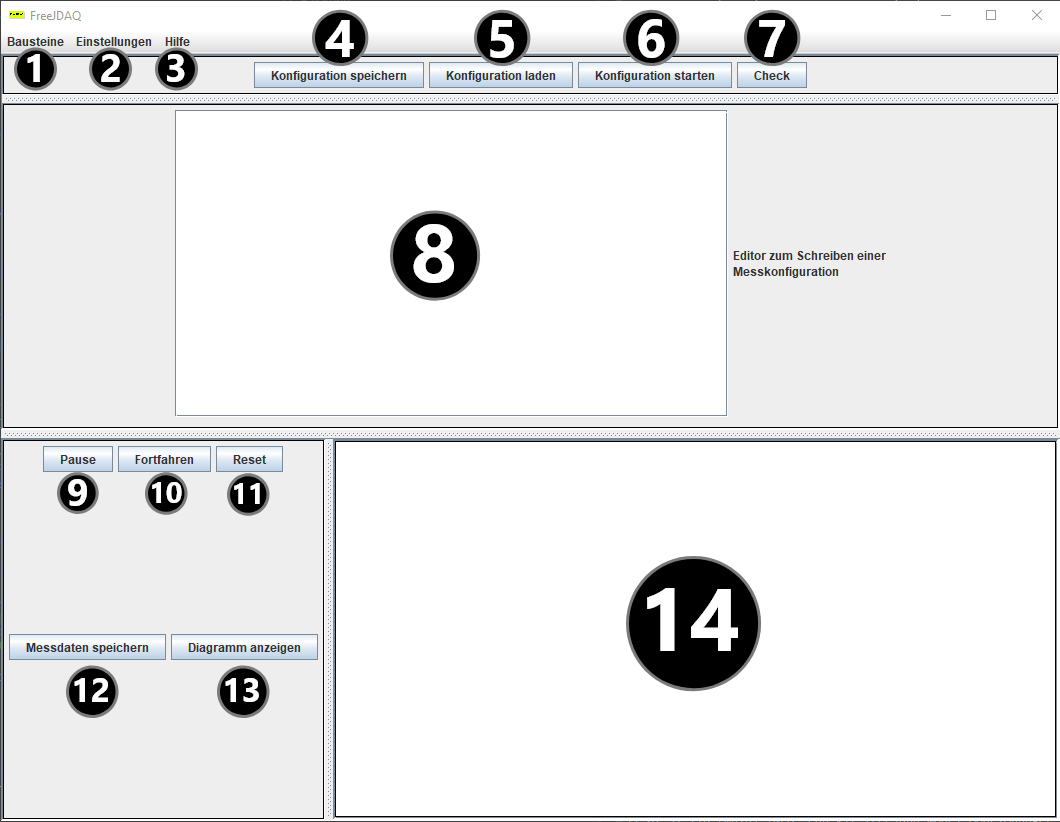
\includegraphics[width = 10cm]{Grafiken/Uebersicht_GUI_Mit_Nummern.png}
        \caption{Die Übersicht über die grafische Benutzeroberfläche von FreeJDAQ. Die Nummern verweißen auf die genauen Beschreibungen, die weiter unten zu finden sind.}
        \label{Uebersicht_GUI_Mit_Nummern}
    \end{center}
\end{figure}

\begin{enumerate}
    \item Bausteine
    \begin{flushleft}
        
\includegraphics[width = 2cm]{Grafiken/1-Bausteine.png}
    \end{flushleft}

    Öffnet ein Fenster, in dem alle verfügbaren Bausteine angezeigt werden. In diesem Fenster können Bausteineigenschaften bearbeitet werden.
    
    \item Einstellungen
    Öffnet ein Fenster, in dem Einstellungen für FreeJDAQ eingesehen werden können. Manche der Einstellungen können angepasst und über den Knopf ''System Einstellungen speichern'' gespeichert werden. Diese beinhalten:
    \begin{itemize}
        \item Fenster-Einstellungen
        \item System-Einstellungen
        \item Messlauf
        \item RasPI
        \item Test Modus
    \end{itemize}
    
    \item Hilfe
    Öffnet ein Fenster, in dem eine Beschreibung der für das Arbeiten mit FreeJDAQ enthalten ist. Hier können folgende Informationen gefunden werden:
    \begin{itemize}
        \item Systemvorraussetzungen
        \item Softwareanforderungen
        \item Tutorials
    \end{itemize}

    \item Konfiguration speichern
    Öffnet ein Fenster um die aktuelle Konfiguration zu speichern. Der Speicherort und der Name der Konfiguration können, in diesem Fenster, festgelegt werden.
    
    \item Konfiguration laden
    Öffnet ein Fenster zum laden einer Konfiguration.
    
    \item Konfiguration starten
    Startet die aktuell verwendete Konfiguration.
    
    \item Check
    Überprüft die aktuell verwendete Konfiguration auf Lauffähigkeit. Im Fehlerfall wird dem Benutzer eine aussagekräftige Fehlermeldung mitgeteilt.
    
    \item Editor für Konfigurationen
    In diesem Feld können Konfigurationen geschrieben werden. Eine Beschreibung der Sprache, zum schreiben einer Konfiguration, kann in der Hilfe gefunden werden.
    
    \item Pause
    Pausiert einen Messlauf nachdem er gestartet wurde.
    
    \item Fortfahren
    Setzt einen pausierten Messlauf fort.
    
    \item Reset
    Setzt einen pausierten Messlauf in den Anfangszustand zurück.
    
    \item Messdaten speichern
    Speichert die Daten, die während des Messlaufs bestimmt wurden, am gewünschten Speicherort.
    
    \item Diagramm anzeigen
    Erstellt ein Diagramm aus den Daten, die während des Messlaufs bestimmt wurden.
    
\end{enumerate}



\begin{flushleft}
    
\includegraphics[width = 2.5cm]{Grafiken/2-Einstellungen.png}
\end{flushleft}

\begin{flushleft}
    
\includegraphics[width = 1cm]{Grafiken/3-Hilfe.png}
\end{flushleft}

\begin{flushleft}
    
\includegraphics[width = 4cm]{Grafiken/4-Konfiguration_speichern.png}
\end{flushleft}

\begin{flushleft}
    
\includegraphics[width = 4cm]{Grafiken/5-Konfiguration_laden.png}
\end{flushleft}

\begin{flushleft}
    
\includegraphics[width = 4cm]{Grafiken/6-Konfiguration_starten.png}
\end{flushleft}

\begin{flushleft}
    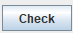
\includegraphics[width = 2cm]{Grafiken/7-Check.png}
\end{flushleft}

\begin{flushleft}
    
\includegraphics[width = 2cm]{Grafiken/8-Editor.png}
\end{flushleft}

\begin{flushleft}
    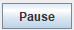
\includegraphics[width = 2cm]{Grafiken/9-Pause.png}
\end{flushleft}

\begin{flushleft}
    
\includegraphics[width = 2cm]{Grafiken/10-Fortfahren.png}
\end{flushleft}

\begin{flushleft}
    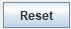
\includegraphics[width = 2cm]{Grafiken/11-Reset.png}
\end{flushleft}

\begin{flushleft}
    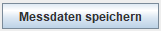
\includegraphics[width = 4cm]{Grafiken/12-Messdaten_speichern.png}
\end{flushleft}

\begin{flushleft}
    
\includegraphics[width = 4cm]{Grafiken/13-Diagramm_anzeigen.png}
\end{flushleft}

\begin{flushleft}
    
\includegraphics[width = 2cm]{Grafiken/14-Datenanzeige.png}
\end{flushleft}

\section{Beschreibung der Messkonfigurationssprache}


Im Folgenden Abschnitt wird erklärt, wie man eine Messkonfiguration erstellt und welche syntaktischen Regeln dabei eingehalten werden müssen.  
schen Aus- und Eingängen.  
 Messkonfiguration über ihren Namen hinzugefügt. Der Name lässt sich über das Systemmenü „Bausteine“ herausfinden.   
gin{itemize}
tbf{blocks: [Baustein1, Baustein2, Baustein3]}
nd Ausgänge repräsentieren Schnittstellen für die Verbindung von 2  
t und kann unter „Bausteine -> Bearbeiten“ eingesehen werden. Daher muss die Anzahl der Ein- und Ausgänge in der Messkonfiguration dieser Anzahl entsprechen. Die Namen sind frei wählbar, aber einen eindeutigen und aussagekräftigen vereinfacht das Schreiben der Konfiguration.  
 ] \textbf{channelListBlock1: [B1out1, B1out2]}
item[ ] \textbf{channelListBlock3: [R1in1, R1in2]} 
 Verbindungen zwischen Ein- und Ausgängen der Bausteine wird ein Datenflussmodel erzeugt, über welches die Messdaten laufen.  Eine Verbindung besteht immer zwischen einem Ausgang und einem Eingang, also einem Tupel aus Ausgang und Eingang.   
spiel für eine solche Konfiguration ist die folgende, welche so in dem Konfigurationsfeld anzeigt werden sollte:
ption{Beispiel Konfiguration im Konfigurationsfeld}


\section{Umgang mit dem Raspberry Pi}

\section{Fehlermeldungen}

Bei Fehlern oder falscher Bedienung der Anwendung werden dem Benutzer Fehlermeldungen angezeigt. Die Fehler unterscheiden sich in 4 Kategorien, welche unten zu sehen sind. Zu jeder Fehlerkategorie gibt es speziellere Fehlerfälle. Diese Fehlerfälle werden in der Fehlerbeschreibung näher beschrieben.

\begin{itemize}


\item[1.] \textbf{Fehler beim Laden einer Konfiguration}: Diese Fehlerkategorie wird gezeigt, wenn es Fehler in der Messkonfiguration gibt.

\item[2.] \textbf{Fehler bei der SSH Verbindung}: Diese Fehlerkategorie wird gezeigt, wenn es zu einem Fehler bei der SSH-Verbindung kommt. Zum Beispiel ist das Passwort oder Benutzername falsch oder es ist keine SSH-Verbindung angelegt.

\item[3.] \textbf{Fehler beim Laden der Bausteine}: Diese Fehlerkategorie wird gezeigt, wenn Bausteine nicht erkannt werden, oder keine ID besitzen.

\item[4.] \textbf{Fehler beim Laden einer Datei}: Diese Fehlerkategorie wird gezeigt, wenn es bei dem Hochladen oder Herunterladen von Dateien von dem Raspberry Pi zu einem Fehler kommt.

\end{itemize}

\section{Limitierung der Anwendung}


\printnoidxglossaries				% generate pdf twice when adding new entries

\end{document}\grid
